\chapter{Distance Oracles}

In this chapter, we learn about distance oracles as presented in the seminal paper \cite{thorup2005approximate}. Distance Oracles are data structures that allow for any undirected graph $G =(V,E)$ to be stored compactly in a format that allows to query for the (approximate) distance between any two vertices $u,v$ in the graph. The main result of this chapter is the following data structure.

\begin{theorem}\label{thm:mainDistanceOracle}
There is an algorithm that, for any integer $k \geq 1$ and undirected graph $G=(V,E)$, computes a data structure that can be stored using $\tilde{O}(kn^{1+1/k})$ bits such that on querying any two vertices $u,v \in V$ returns in $O(k)$ time a distance estimate $\widetilde{\mathbf{dist}}(u,v)$ such that
\[
\mathbf{dist}(u,v) \leq \widetilde{\mathbf{dist}}(u,v) \leq (2k-1) \cdot \mathbf{dist}(u,v).
\]
The algorithm computes the data structure in expected time $\tilde{O}(kmn^{1/k})$.
\end{theorem}

\begin{remark}Note that for $k=1$, the theorem above is trivial: it can be solved by computing APSP and storing the distance matrix of $G$.
\end{remark}

\begin{remark}
We point out that given space $O(n^{1+1/k})$, approximation $(2k-1)$ is the best that we can hope for according to a popular and widely believed conjecture that essentially says that there are unweighted graphs that have no cycle of length $(2k+1)$ but have $\tilde{\Omega}(n^{1+1/k})$ edges. A more careful analysis than we will carry out allows to shave all logarithmic factors from \Cref{thm:mainDistanceOracle} and therefore the data structure is only a factor $k$ off in space from optimal while also answering queries \emph{extremely} efficiently. It turns out that the factor $k$ can also be removed in space and query time (although currently preprocessing is quite expensive), see therefore the following (really involved) articles \cite{chechik2014approximate, chechik2015approximate}.
\end{remark}

\begin{remark}
Also note that in directed graphs no such distance oracle is possible. Even maintaining the transitive closure (the information of who reaches who) can only be preserved if one stores $\tilde{\Omega}(n^2)$ bits.
\end{remark}

\section{Warm-up: A Distance Oracle for $k=2$}

Let us first describe the data structure for the case where $k=2$. See therefore the pseudo-code below. Here we use the convention that $\mathbf{dist}(x,X)$ for some vertex $x \in V$ and some subset $X \subseteq V$ is the minimum distance from $x$ to any $y \in X$, formally $\mathbf{dist}(x,X) = \min_{y \in X} \mathbf{dist}(x,y)$.

\begin{algorithm}
  \SetAlgoLined
  Obtain $S$ by sampling every vertex $v \in V$ i.i.d. with probability $n^{-1/2}$\;
  \ForEach{$s \in S$}{
    Compute all distances from $s$ to any other vertex $v \in V$\;
    In a hash table $\mathcal{H}_s$ store for each $v \in V$ an entry with key $v$ and value $\mathbf{dist}_G(s,v)$.
  }
  
  \ForEach{$u \in V \setminus S$}{
    Find the \emph{pivot} $p(u)$ of $u$ to be some vertex in $S$ that minimizes the distance to $u$\;
    Store $p(u)$ along with $\mathbf{dist}_G(u,p(u)) = \mathbf{dist}_G(u,S)$\;
    Find the \emph{bunch} $B(u) = \{ v \in V \;|\; \mathbf{dist}_G(u,v) < \mathbf{dist}_G(u,S)\}$\;
    In a hash table $\mathcal{H}_u$ store for each $v \in B(v)$ an entry with key $v$ and value $\mathbf{dist}_G(u,v)$.
  }
  \caption{\textsc{Preprocess}(G)}
\end{algorithm}

The key to the algorithm is the definition of \emph{pivots} and \emph{bunches}. Below is an example that illustrates their definitions.

\begin{figure}[!ht]
    \centering
    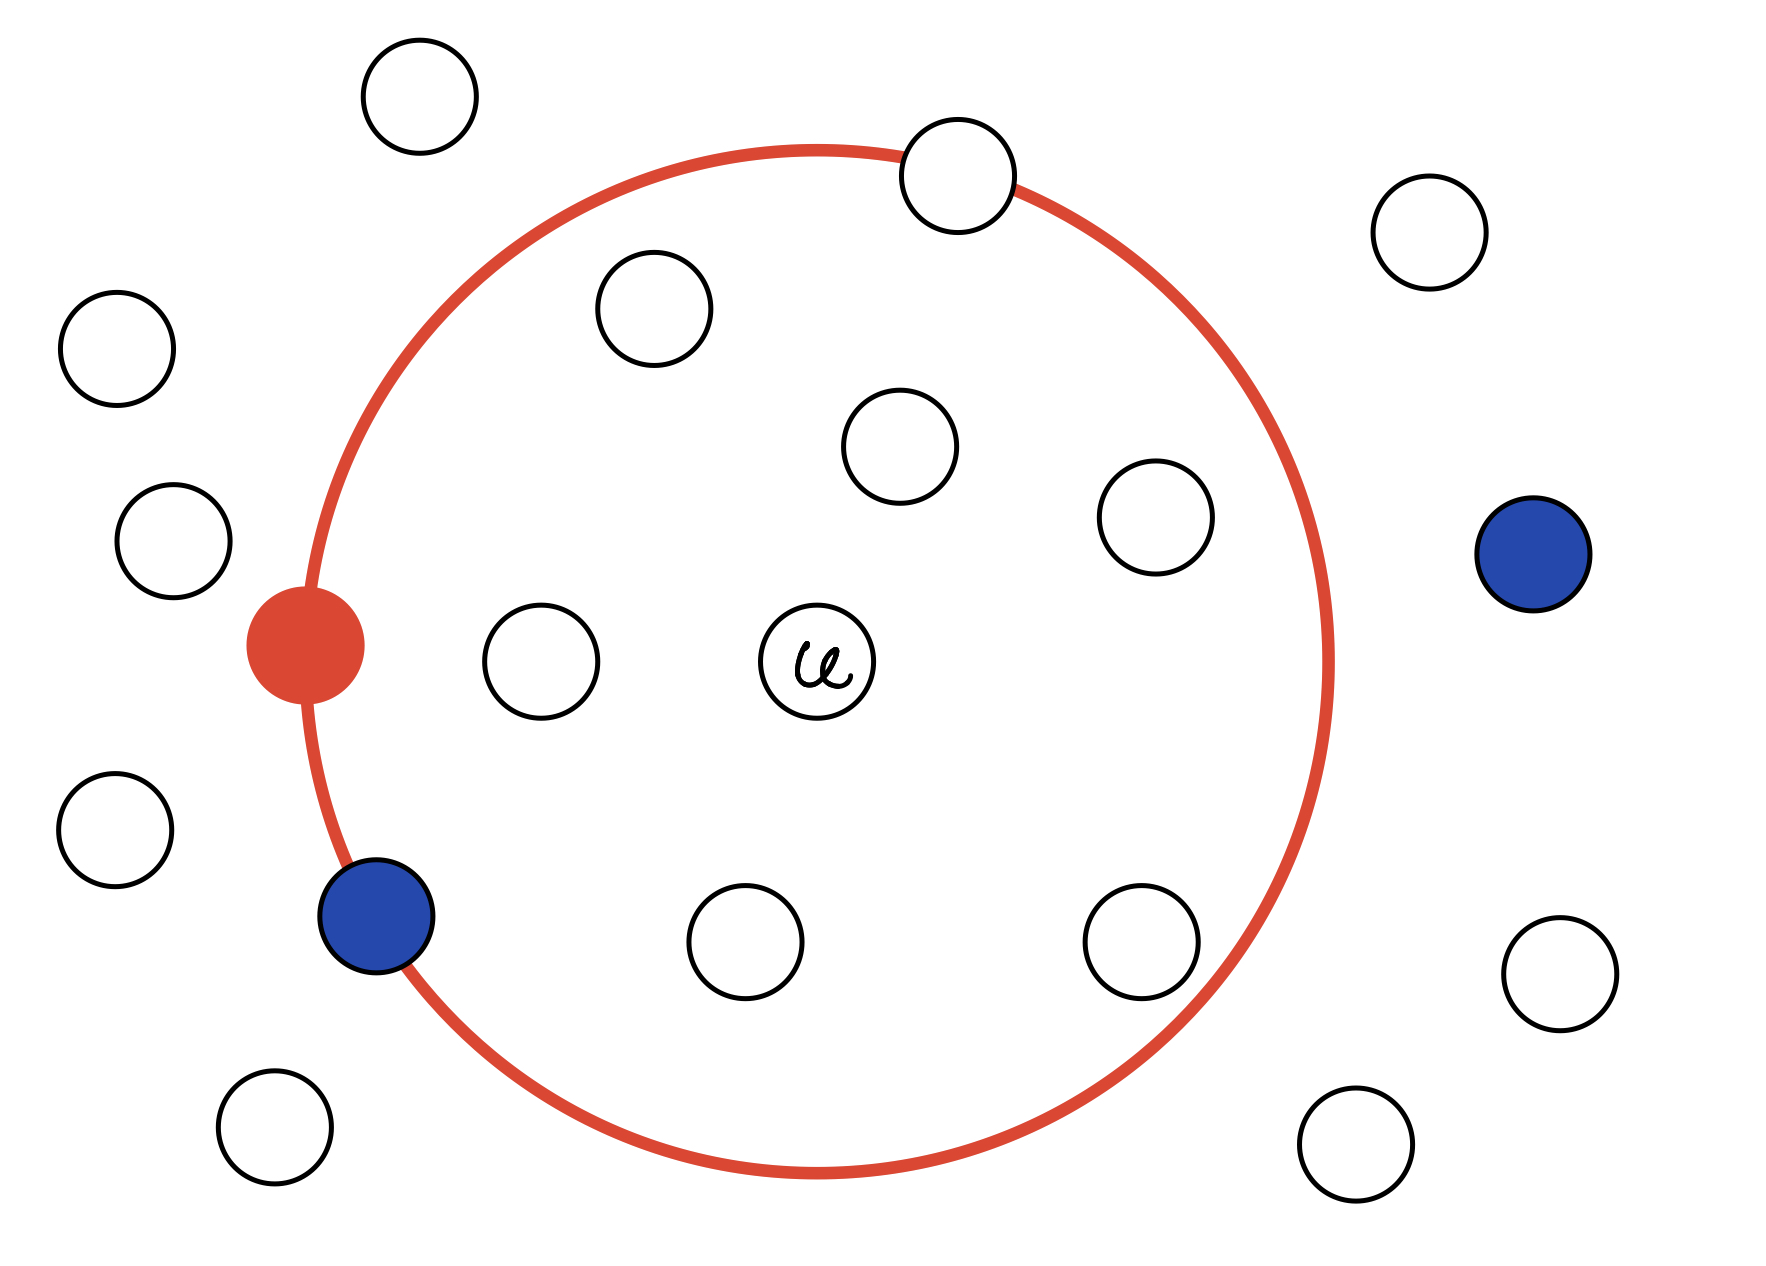
\includegraphics[scale=0.2]{./fig/lecture_DistanceOracles_Bunch.jpeg}
    \caption{Graph $G$ (without the edges) where vertices are drawn according to their distance from $u$. The blue and red vertices are in $S$. The red vertex is chosen to be the pivot $p(u)$. Note that another vertex in $S$ could have been chosen to become the pivot. The bunch of $u$ is the vertices that are strictly withing the red circle. In particular, both blue vertices, the red vertex and also the white vertex on the boundary of the red circle are \emph{not} in the bunch $B(u)$.}
\end{figure}

Without further due, let us discuss the query procedure which is depicted below. It essentially consists of checking whether the vertex $v$ is already in the bunch of $u$ in which case we have stored the distance $\mathbf{dist}_G(u,v)$ explicitly. Otherwise, it uses a detour via its pivot.

\begin{algorithm}
  \SetAlgoLined
  \lIf{$v \in \mathcal{H}_u$}{
    \Return value $\mathbf{dist}_G(u,v)$
  }
  \Return $\mathbf{dist}_G(u,p(u)) + \mathbf{dist}_G(p(u),v)$ (the latter from $\mathcal{H}_{p(u)}$)
  \caption{\textsc{Query}(u,v)}
\end{algorithm}

The second case is illustrated below.

\begin{figure}[!ht]
    \centering
    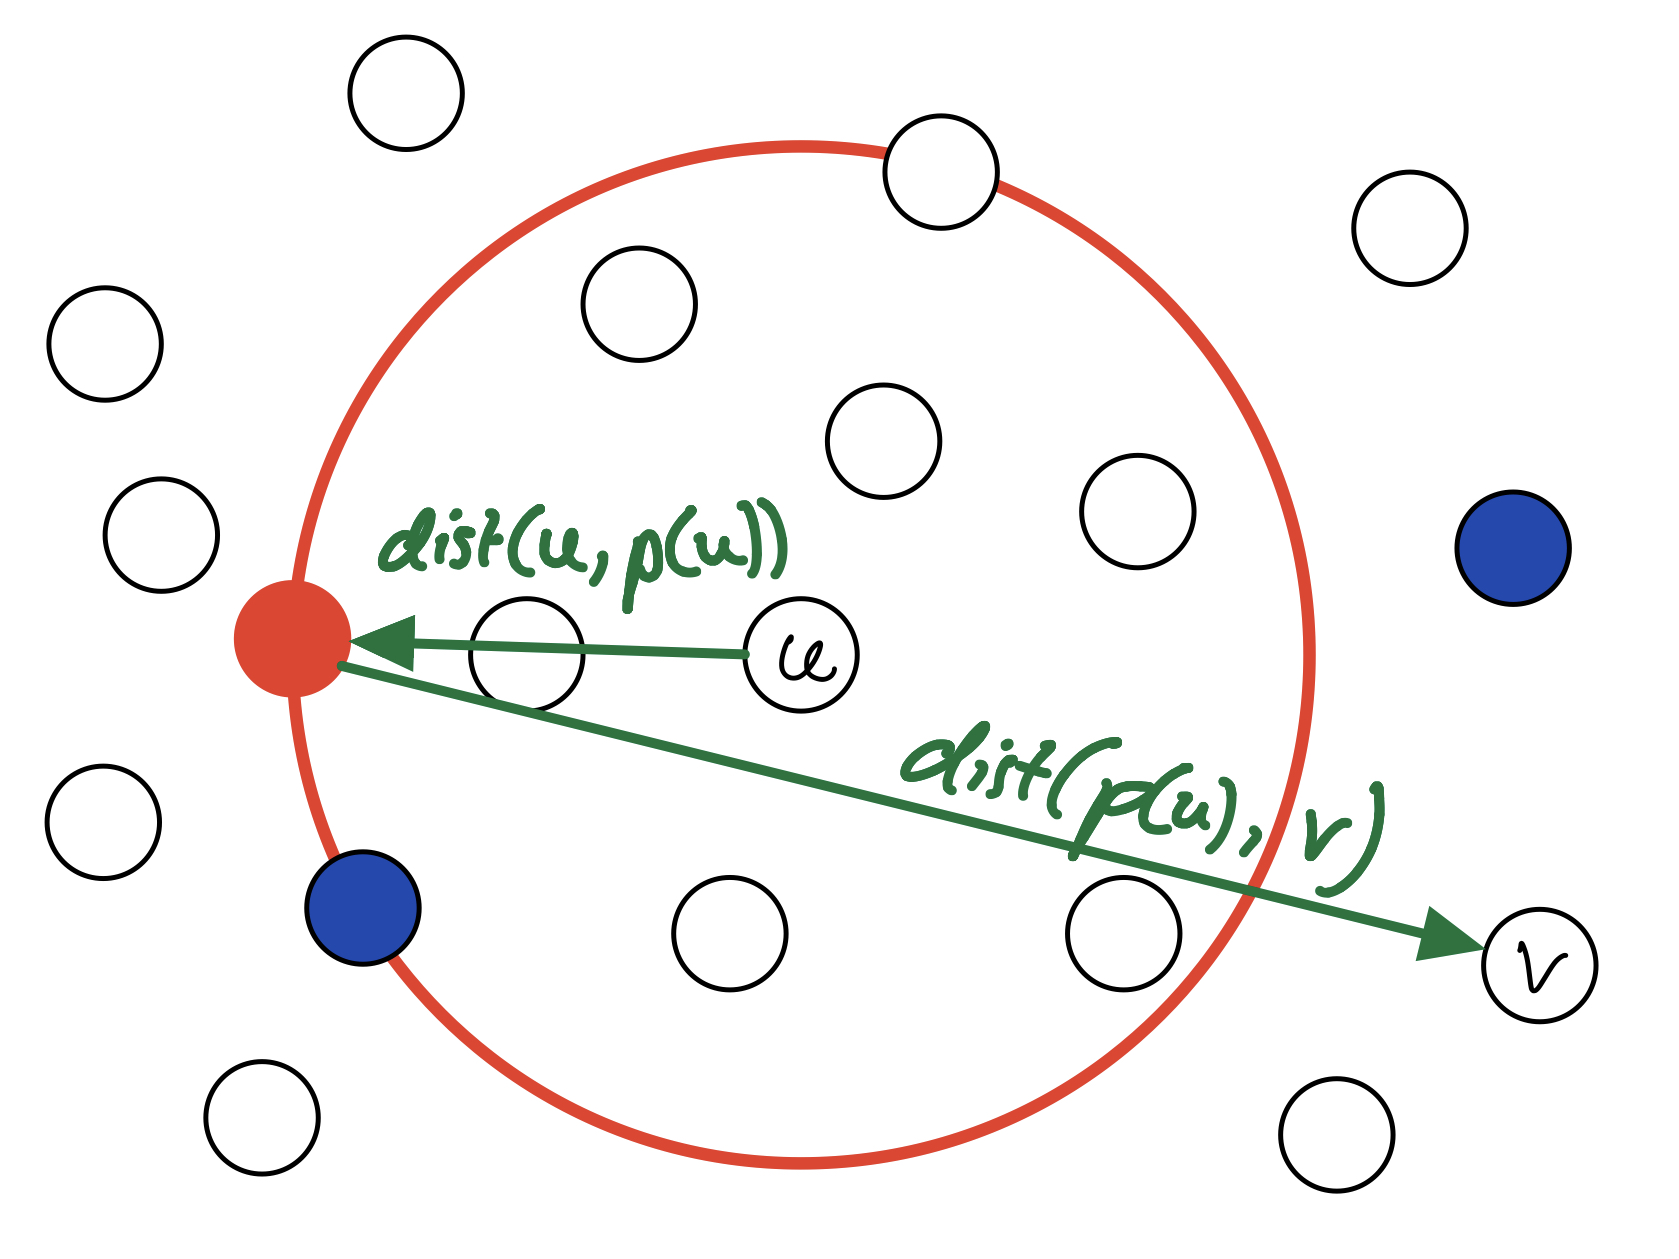
\includegraphics[scale=0.25]{./fig/lecture_DistanceOracles_Query.jpeg}
\end{figure}

\paragraph{Approximation Analysis.} It is straight-forward to see that if we return in line 1 of the query algorithm, then we return the exact distance.

If we return in the second line, then we know that $v \not\in B(u)$. By definition of a bunch this implies that 
\[
 \mathbf{dist}(u,v) \geq \mathbf{dist}(u,S) = \mathbf{dist}(u,p(u)).
\]
We can further use the triangle inequality to conclude that
\[
\mathbf{dist}_G(p(u),v) \leq \mathbf{dist}(u,p(u)) + \mathbf{dist}(u,v)
\]
Combining these two inequalities, we obtain
\[
\mathbf{dist}_G(u,p(u)) + \mathbf{dist}_G(p(u),v) \leq 2 \cdot \mathbf{dist}(u,p(u)) + \mathbf{dist}(u,v) \leq 3 \cdot \mathbf{dist}(u,v).
\]
We conclude that we obtain a $3$-approximation.

\paragraph{Space Analysis.} For each vertex $s \in S$, we store a hash-table with one entry for each vertex $v$. This can be stored with space $O(|S|n)$. We have by a standard Chernoff-bound that $|S| = \tilde{O}(\sqrt{n})$ w.h.p. so this becomes $\tilde{O}(n^{3/2})$.

Next, fix some $u \in V \setminus S$, and let us argue about the size of $B(u)$ (which asymptotically matches $|\mathcal{H}_u|$). We order the vertices $v_1, v_2, \dots, v_n$ in $V$ by their distance from $u$. Since we sample uniformly at random, by a simple Chernoff bound, we obtain that the first vertex $v_i$ in $v_1, v_2, \dots, v_n$ that is in $S$ has $i = \tilde{O}(\sqrt{n})$ w.h.p.. But note that since only vertices that are \emph{strictly} closer to $u$ than $v_i$ are in $B(u)$, this implies that $|B(u)| = \tilde{O}(\sqrt{n})$.

It remains to take a careful union bound over all bad events at every vertex $u \in V \setminus S$ to conclude that with high probability, the hash tables $\mathcal{H}_u$ for all $u \in V \setminus S$ combined take total space $\tilde{O}(|V \setminus S| \sqrt{n}) = \tilde{O}(n^{3/2})$. For the rest of the section, we condition on the event that each $|B(v)| =\tilde{O}(\sqrt{n})$ to use it as if it was a deterministic guarantee.

\paragraph{Preprocessing and Query Time.} In order to find the distances stored in the hash tables $\mathcal{H}_s$ for $s \in S$, we can simply run Dijkstra from each $s \in S$ on the graph in total time $\tilde{O}(m|S|) = \tilde{O}(mn^{1/2})$.

To compute the \emph{pivots} for each vertex $u$, we can insert a super-vertex $s'$ and add an edge from $s'$ to each $s \in S$ of weight $0$. We can then run Dijkstra from $s'$ on $G \cup \{s'\}$. Note that for each $u$, we have $\mathbf{dist}_{G \cup \{s'\}}(s', u) = \mathbf{dist}_G(p(u),u)$ and that $p(u)$ can be chosen to be the closest vertex on the path from $s'$ to $u$ that Dijkstra outputs along with the distances (recall that Dijkstra can output a shortest path tree). This takes $\tilde{O}(m)$ time.

It remains to compute the bunches $B(u)$. Here, we use duality: we define the cluster $C(w)$ for every vertex $w \in V \setminus S$ to be the set
\[
    C(w) = \{ v \in V \;|\; \mathbf{dist}_G(v,w) < \mathbf{dist}_G(v,p(v))\}.
\]
Note the subtle difference to the bunches in that membership of $v$ now depends on $p(v)$ and \emph{not} on $p(u)$! It is not hard to see that $u \in C(w) \iff w \in B(u)$. And it is straight-forward to compute the bunches from the clusters in time $O(\sum_v |B(v)|) = O(\sum_w |C(w)|) = \tilde{O}(n^{3/2})$. 

Finally, it turns out that we can compute each $C(w)$ by running Dijkstra with a small modification.

\begin{lemma}[Lemma 4.2 in \cite{thorup2005approximate}]
Consider running Dijkstra from a vertex $w$ but only relaxing edges incident to vertices $v$ that satisfy $\mathbf{dist}_G(v,w) < \mathbf{dist}_G(v,p(v))$. Then, the algorithm computes $C(w)$ and all distances $\mathbf{dist}(v,w)$ for $v \in C(w)$ in time $\tilde{O}(|E(C(w))|)$ where $E(C(w))$ are the edges that touch a vertex in $C(w)$. 
\end{lemma}
 
It remains to observe that the total time required to compute all clusters is
\[
    \tilde{O}(\sum_{w} |E(C(w))|) = \tilde{O}(\sum_{w, v \in C(w)} |E(v)|) = \tilde{O}(\sum_{v, w \in B(v)} |E(v)|) = \tilde{O}(\sum_{v} |E(v)| |B(v)|).
\]
But we have upper bounded $|B(v)| = \tilde{O}(\sqrt{n})$ for all $v$, thus each vertex just pays its degree $\tilde{O}(\sqrt{n})$ times and we get running time $\tilde{O}(m\sqrt{n})$.

\paragraph{Monte Carlo vs. Las Vegas.} Note that the analysis above only guarantees that the algorithm works well with high probability. However, it is not hard to see that the algorithm can be transformed into a Las Vegas algorithm: whenever we find a bunch $B(v)$ whose size exceeds our $\tilde{O}(\sqrt{n})$ bound, we simply re-run the algorithm. This guarantees that the final data structure that we output indeed satisfies the guarantees stipulated in the theorem.

\section{Distance Oracles for any $k \geq 2$}

The generalization for all $k$'s is rather straight-forward except for the query operation which works a bit magically. Let's first define the data structure by giving our new pre-processing algorithm.

\begin{algorithm}
  \SetAlgoLined
  $S_1 = V$; $S_{k+1} = \emptyset$\;
  \lForEach{$i \in [1,k]$}{
    Obtain $S_{i+1}$ by sampling every $v \in S_{i}$ i.i.d. with prob. $n^{-1/k}$
  }
  
    \ForEach{$u \in V$}{
        \ForEach{$i \in [1,k]$}{Let $p_{i}(u)$ be some vertex in $S_{i}$ that minimizes the distance to $u$\;
        Store $p_{i}(u)$ along with $\mathbf{dist}_G(u,p_{i}(u))$. }
        Let \emph{bunch} $B(u) = \bigcup_i B_i(u)$ where $B_i(u) = \{ v \in S_i \;|\; \mathbf{dist}_G(u,v) < \mathbf{dist}_G(u,S_{i+1})\}$\;
        In a hash table $\mathcal{H}_u$ store for each $v \in B(u)$ an entry with key $v$ and value $\mathbf{dist}_G(u,v)$.
     }
  \caption{\textsc{Preprocess}(G)}
\end{algorithm}

Note that in a sense this algorithm is almost easier than the one for $k=2$ since it treats each level in the same fashion. Here we ensure that the last set $S_{k+1}$ is empty (which would happen with constant probability otherwise). 

We make the implicit assumption throughout that $S_k \neq \emptyset$ so that $p_k(u)$ is well-defined for each $u$. We also define $\mathbf{dist}(x,X) = \infty$ if $X$ is the empty set.

The drawing below illustrates the new definition of a bunch where we have chosen $k=3$ to keep things simple.

\begin{figure}[!ht]
    \centering
    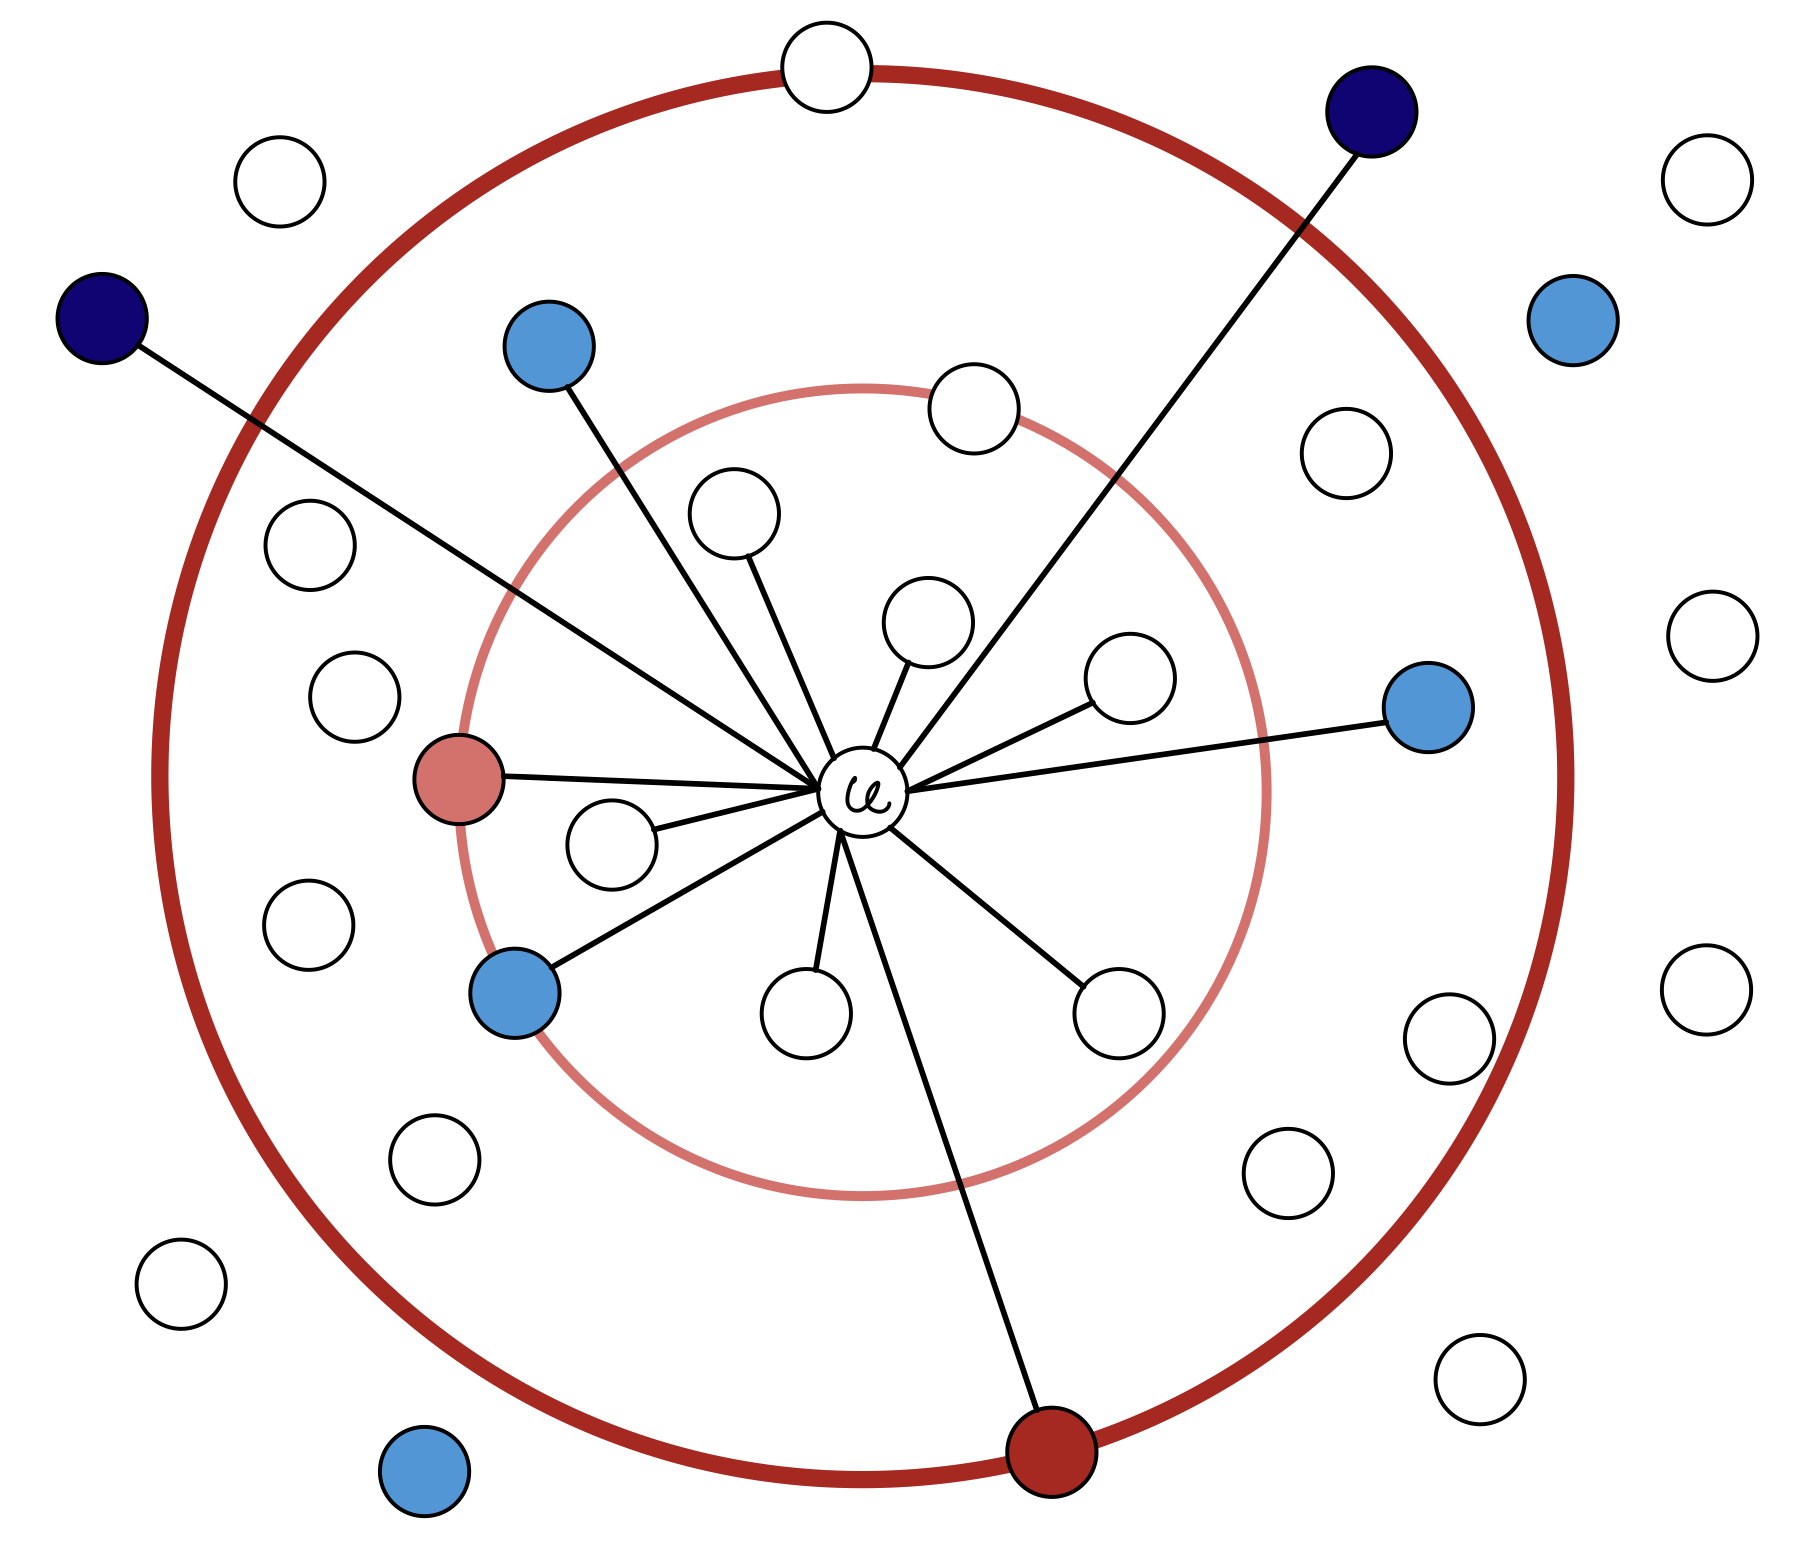
\includegraphics[scale=0.25]{./fig/lecture_DistanceOracles_MultiLevelBunch.jpg}
    \caption{Graph $G$ (without the edges) where vertices are drawn according to their distance from $u$. All vertices are in $S_1$. The blue and red vertices are in $S_2$. The dark blue and dark red vertices are also in $S_3$. Finally, we have $S_4 = \emptyset$. 
    The light red vertex is chosen as pivot $p_2(u)$; the dark red vertex is chosen as pivot $p_3(u)$. 
    The bunch $B(u)$ includes all vertices that have a black edge in this graph to $u$; in particular these are the white vertices within the circle drawn in light red ($B_1(u)$); the light blue vertices encircled by the dark red circle ($B_2(u)$); and all dark blue vertices ($B_3(u)$).}
\end{figure}

Before we explain the query procedure, let us give a (rather informal) analysis of the space required by our new data structure.

\paragraph{Space Analysis.} We have for each vertex $u \in V$, and each $1 \leq i \leq k$ that the bunch $B_i(u)$ consists of all vertices in $S_i$ that are closer to $u$ than the closest vertex in $S_{i+1}$. 

Now, order the vertices $x_1, x_2, \dots$ in $S_i$ by their distance from $u$. Since each vertex in $S_i$ is sampled into $S_{i+1}$ with probability $n^{-1/k}$, we have that with high probability some vertex $x_i$ with $i = O(n^{1/k} \log n)$ is sampled into $S_{i+1}$. This ensures that $|B_i(u)| = \tilde{O}(n^{1/k})$ with high probability. 

Applying this argument for all $i$, we have that $|B(u)| = \tilde{O}(k \cdot n^{1/k})$ for each $u$ w.h.p. and therefore our space bound follows.

\paragraph{Preprocessing Time.} Much like in the $k=2$ construction, we can define for each $u \in S_i \setminus S_{i+1}$ the cluster $C(u) = \{ v \in V \;|\; \mathbf{dist}_G(u,v) < \mathbf{dist}_G(v,S_{i+1})\}$. Extending our analysis from before using this new definition, we get construction time $\tilde{O}(kmn^{1/k})$.

\paragraph{Query Operation.} A straight-forward way to query our new data structure for a tuple $(u,v)$ would be to search for the smallest $i$ such that $v \in B(p_i(u))$ and then return $\mathbf{dist}_G(u, p_i(u)) + \mathbf{dist}_G(p_i(u), v)$. This can be analyzed in the same way as we did for $k=2$ to obtain stretch $4k-3$\footnote{One can actually prove that this strategy gives an $4k-5$ stretch with a little trick.}.

However, we aim for stretch approximation $2k-1$. We state below the pseudo-code to achieve this guarantee.

\begin{algorithm}
  \SetAlgoLined
  $w \gets u$; $i \gets 1$\;
  \While{$w \not\in B(v)$}{
    $i \gets i+1$\;
    $(u,v) \gets (v,u)$\;
    $w \gets p_i(u)$
  }
  \Return $\mathbf{dist}_G(u,w) + \mathbf{dist}_G(w,v)$
  \caption{\textsc{Query}(u,v)}
\end{algorithm}

Our main tool in the analysis is the claim below where we define $\Delta = \mathbf{dist}_G(u,v)$. 

\begin{claim}\label{claim:DistanceOracleSwapping} After the $i^{th}$ iteration of the while-loop, we have $\mathbf{dist}_G(u,w) \leq i\Delta$.
\end{claim}

This implies our theorem, since we have at most $k-1$ iterations, then $w$ is a vertex in $S_k$ and $S_k \subseteq B(x)$ for all vertices $x \in V$. Therefore we have that for the final $w$, we have $\mathbf{dist}_G(u,w) \leq (k-1)\Delta$. It remains to conclude by the triangle inequality that 
\[
\mathbf{dist}_G(u,w) + \mathbf{dist}_G(w,v) \leq 2\mathbf{dist}_G(u,w) + \Delta \leq (2k-1)\mathbf{dist}_G(u,v).
\]

\begin{proof}[Proof of Claim~\ref{claim:DistanceOracleSwapping}]
Let $w_i, u_i, v_i$ denote the variables $w,u,v$ after the $i^{th}$ while-loop iteration (or right before for $w_0,u_0,v_0$).

For $i = 0$, we have that $w_0 = u_0$; thus, $\mathbf{dist}_G(u_0,w_0) = 0$.

For $i \geq 1$, we want to prove that if the $i^{th}$ while-loop iteration is executed then $\mathbf{dist}_G(u_i,w_i) \leq \mathbf{dist}_G(u_{i-1},w_{i-1}) + \Delta$ (if it is not executed then the statement follows trivially).

In order to prove this, observe that by the while-loop condition, we must have had $w_{i-1} \not\in B(v_{i-1})$, thus  $\mathbf{dist}_G(v_{i-1}, w_{i-1}) \geq \mathbf{dist}_G(v_{i-1}, p_i(v_{i-1}))$.

But the while-iteration sets $u_i = v_{i-1}$ and $w_i = p_i(v_{i-1})$, and therefore we have
\begin{align*}
\mathbf{dist}_G(u_{i}, w_i) &= \mathbf{dist}_G(v_{i-1}, p_i(v_{i-1})) \\
&\leq
\mathbf{dist}_G(v_{i-1}, w_{i-1}) \\
&\leq \mathbf{dist}_G(u_{i-1}, w_{i-1}) + \mathbf{dist}_G(v_{i-1}, u_{i-1}) \\ &= \mathbf{dist}_G(u_{i-1}, w_{i-1}) + \Delta.
\end{align*}
\end{proof}